\documentclass[11pt,letterpaper]{article}

\input{../../../../.config/latex/preamble_v1.tex}

\lightmode

\title{\textbf{Math 55b Final Exam}}

\begin{document}
\maketitle

\begin{center}
    \textit{I affirm my awareness of the standards of the Harvard College Honor Code. While completing this exam, I have not consulted any external sources other than class notes and the textbooks. I have not discussed the problems or solutions of this exam with anyone, and will not discuss them until after the due date.} 

    \textit{Signed: \und{Lev Kruglyak}}
\end{center}

\begin{problem}
    Let $(X,d)$ be a compact metric space, and let $U\subset X\times X$ be an open subset of $X\times X$ (with the product topology) which contains the diagonal $\Delta=\{(p,p)\,|\,p\in X\}$.
    \begin{enumerate}[(a)]
        \item Show that there exists $\epsilon>0$ such that $U$ contains $V_\epsilon=\{(p,q)\in X\times X\,|\,d(p,q)<\epsilon\}$.
        \item Show that this conclusion may be false if we drop the assumption that $X$ is compact.
    \end{enumerate}
\end{problem}

\begin{solution}
    \textbf{(a)} For each $x\in X$, let $\epsilon_x>0$ be some radius such that $B_{\epsilon_x}(x,x)\subset U$. Such $\epsilon>0$ is guaranteed to exist because $\Delta\subset U$ and using the definition of an open set. Thus we have an open cover of $X\times X$:
    \[
        X\times X = (X\times X \setminus \Delta)\cup\bigcup_{x\in X} B_{\epsilon_x}(x,x).
    \] 
    ($\Delta$ is clearly closed so $X\times X\setminus \Delta$ is open.) Since $X\times X$ is compact, there must be some finite subcover which still covers the whole space. So we actually have some finite set of $x_1,\ldots,x_{n}\in X$ such that
    \[
        X\times X=(X\times X\setminus \Delta)\cup \bigcup_{1\leq i \leq n} B_{\epsilon_{x_n}}(x_n,x_n).
    \] 
    Notice that $\Delta\subset\bigcup_{1\leq i \leq n} B_{\epsilon_{x_n}}(x_n, x_n)\subset U$. Let $\delta>0$ be a Lebesgue number for this cover. Then by definition of a Lebesgue number, for any $x\in X$, $B_{\delta}(x,x)$ must lie inside one of the sets in the cover. So we have \[\Delta \subset \bigcup_{x\in X} B_{\delta}(x,x) \subset \bigcup_{1\leq i \leq n} B_{\epsilon_{x_n}}(x_n, x_n)\subset U.\]
    Finally we notice that for any point $(x,y)\in X\times X$, if $d(x,y)<\delta$, then $d((x,x), (x,y))\leq \|(0,\delta)\|=\delta$. So $V_\delta \subset \bigcup_{x\in X} B_\delta(x,x)\subset U$ and we are done.

    \textbf{(b)} Let $X=[0,1)$ be a (non-compact) subset of the unit interval with the usual Euclidean metric. Consider the open subset $U\subset X\times X$ defined by
    \[
        U=\{(x,y)\in X\times X\mid 2x-1 < y < x/2+1/2\}.
    \] 
    Since $2x-1 < x < x/2 + 1/2$ whenever $x\in [0,1)$, it's clear that $\Delta\subset U$ so $U$ satisfies the conditions of the problem. Geometrically, this set looks like the shaded gray region:
    \begin{center}
        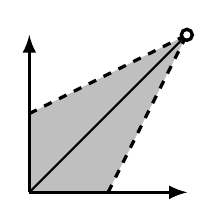
\begin{tikzpicture}[very thick]
            \fill[fill=gray!50] (0,1) -- (2,2) -- (1,0) -- (0,0) -- cycle;
            \draw[-latex] (0,0) -- (0,2);
            \draw[-latex] (0,0) -- (2,0);
            \draw[-latex] (0,0) -- (2,0);
            \draw[-, thick] (0,0) -- (2,2);

            \draw[dashed] (1,0) -- (2,2);
            \draw[dashed] (0,1) -- (2,2);

            \draw[fill=white] (2,2) circle (0.07);
        \end{tikzpicture}
    \end{center}
    We claim that there does not exist an $\epsilon>0$ such that $V_\epsilon \subset U$. To prove this, suppose for the sake of contradiction that there is some $\epsilon>0$ such that $V_\epsilon \subset U$. Let $x=1-\epsilon$. Then 
    \[
        d\left(x, \frac{x}{2}+\frac12\right) = \frac{x}{2}+\frac12 - x = -\frac{x}{2}+\frac{1}{2} \leq \frac{\epsilon}{2}<\epsilon
    \] 
    so $(x, x/2+\frac12)\in U$, which is a contradiction since $x/2+1/2\not< x/2+1/2$.
\end{solution}

\begin{problem}
    Recall that a {\em retraction} of a topological space $X$ onto a subspace $A\subset X$ is a continuous map $r:X\to A$ such that $r(a)=a$ for all $a\in A$. We consider the M\"obius strip $$X=(I\times I)/\sim \quad\textrm{where}\quad (0,y)\sim (1,1-y) \quad \forall y\in I,$$ where $I=[0,1]$, and its ``boundary'' $A=(I\times \{0,1\})/\!\sim$ (the image in $X$ of the two edges of the square that don't get identified with each other by the quotient map). Show that there does not exist a retraction of the M\"obius strip $X$ onto its boundary $A$.
\end{problem}

\begin{solution}
    Suppose for the sake of contradiction that there was a retraction of the M\"obius strip $M$ onto its boundary $\partial M$. Let $H$ be the half circle $\{(x,1/2)\mid x\in [0,1]\}/\sim$ which goes around the center of the M\"obius strip. We have the sequence of maps:
    \[
        \partial M \xrightarrow[]{\;\;p\;\;} H \xrightarrow[]{\;\;i\;\;} M
    \] 
    where $p : \partial M \to H$ sends $(x,y) \mapsto (x,1/2)$ and $i$ is the obvious inclusion map. Since $(1,y)$ and $(0,1-y)$ map to the same element under $p$, it is fairly easy to show that $p$ is actually a $2$-sheeted covering map, and since $\partial M$ is path connected it follows that
    \[
        [\pi_1(H, p(x_0)) : p^*(\pi_1(\partial M, x_0)] = |p^{-1}(p(x_0))| = 2
    \] 
    for any $x_0\in \partial M$, so $\pi_1(\partial M)$ is an index $2$ subgroup of $\pi_1(H)$. Next we can show that $H$ is actually a deformation retract of $M$ by the homotopy $H : M \times [0,1] \to M$ given by $H((x,y), t) = (x,(1-t)y+t/2)$. So the inclusion map $i$ induces an isomorphism $i^* : \pi_1(H) \to \pi_1(M)$. 
    Thus $(i\circ p)^*(\pi_1(\partial M))$ is an index $2$ subgroup of $\pi_1(M)$.

    Now let $r : M \to \partial M$ be the retraction. By functoriality, it follows that $r^* : \pi_1(M) \to \pi_1(\partial M)$ is injective. So we have the maps
    \[
        \pi_1(\partial M) \xrightarrow[]{\;\;i^*\circ p^*\;\;} \pi_1(M) \xrightarrow[]{\;\;r^*\;\;} \pi_1(\partial M).
    \] 
    Note that $\partial M$ is a circle, and $M$ deformation retracts onto the half circle $H$, so the fundamental groups $\pi_1(\partial M)$ and $\pi_1(M)$ are both infinite cyclic groups, i.e. isomorphic to $\Z$. Let $b\in \pi_1(\partial M)$ and $m\in \pi_1(M)$ be generators. Then $(i\circ p)^*(b) = \pm 2m$ since it is an index $2$ subgroup. Since $r\circ i = \textrm{id}_{\partial M}$, we have $r^*\circ i^* = \textrm{id}_{\partial M}$, so $r^*\circ i^*\circ p^*(b) = p^*(b)=b$ but also equals $r^*(\pm 2m)=\pm 2r^*(m)$. Since $r^*(m)\in \pi_1(\partial M)$, we must have $r^*(m)=nb$ for some $n$. But then $\pm 2r^*(m)=\pm 2nb = b$ which is impossible, so we have our contradiction.
\end{solution}

\begin{problem}
    Let $S^n=\{(x_1,\dots,x_{n+1})\in \R^{n+1}\,|\,\sum x_i^2=1\}$ be the unit sphere in $\R^{n+1}$, and for $k<n$ let $S^k$ be the unit sphere in the $(x_1,\dots,x_{k+1})$-coordinate plane, i.e.\ $$S^k=\{(x_1,\dots,x_{n+1})\in S^n\,|\,x_{k+2}=\dots=x_{n+1}=0\}.$$ Determine the fundamental group $\pi_1(S^n\setminus S^k)$. 
\end{problem}

\begin{solution}
    We'll first prove a lemma relevant to this problem:
    \begin{ilemma}
        For any $n>0$ and $k<n$, we have the homotopy equivalence
        \[
            S^n\setminus S^k\simeq S^{n-k-1}
        \] 
        where $S^k$ is embedded into $S^n$ in the obvious way as described in the problem.
    \end{ilemma}
    \begin{proof}
        In this proof, it will be useful to make a distinction between different ways of embedding $S^k$ into $S^n$. So let $\iota_1 : S^k \to S^n$ be defined in the same way as in the problem, i.e. $\iota_1(x_1,\ldots,x_{k+1}) = (x_1,\ldots,x_{k+1}, 0, \ldots, 0)\in S^n$. Next, we will consider the embedding $\iota_2 : S^{n-k-1} \to S^n$ given by $\iota_2(x_1,\ldots,x_{n-k}) = (0, \ldots, 0, x_1,\ldots,x_{n-k})$. (i.e. the first $k+1$ entries are zero) We claim that $\iota_2(S^{n-k-1})$ is a deformation retraction of $S^n\setminus\iota_1(S^k)$. (Note that $\iota_2(S^{n-k-1})\cap \iota_1(S^k)=\emptyset$. Consider the homotopy $F : (S^n\setminus \iota_1(S^k))\times [0,1] \to S^n\setminus \iota_1(S^k)$ given by 
        \[
            F((x_1,\ldots,x_{n+1}), t) = \frac{((1-t)x_1,\ldots,(1-t)x_{k+1}, x_{k+2}, \ldots, x_{n+1})}{\|((1-t)x_1,\ldots,(1-t)x_{k+1}, x_{k+2}, \ldots, x_{n+1})\|}.
        \] 
        To see why this function is continuous, note that the only way the fraction would be undefined/discontinuous would be if $\|((1-t)x_1,\ldots,(1-t)x_{k+1},x_{k+2},\ldots,x_{n+1})\|=0$. If $t\neq 1$, this would only happen if $x_1=x_2=\cdots=x_{n+1}=0$, which is impossible since $\sum^{n+1}_{i=1} x_i^2=1$. If $t=1$, then
        \[
            \|((1-t)x_1,\ldots,(1-t)x_{k+1},x_{k+2},\ldots,x_{n+1})\|=\|(0,\ldots,0,x_{k+2},\ldots,x_{n+1})\|\neq 0
        \] 
        because not all $x_{k+2}, \ldots, x_{n+1}$ can be zero. (Recall that our input space is $S^n\setminus \iota_1(S^k)$. So this is a continuous, defined map. To see why its a homotopy, note that $F((x_1,\ldots,x_{n+1}, 0) = (x_1,\ldots,x_{n+1})$, and $F((x_1,\ldots,x_{n+1}), 1) = \iota_2(x_{k+2},\ldots,x_{n+1})$. Lastly, $F(\iota_2(x_{1},\ldots,x_{n-k}), t) = \iota_2(x_{1}, \ldots, x_{n-k})$ for any $t\in [0,1]$. This completes the proof of the deformation retraction, which is a homotopy equivalence of the spaces in question.
    \end{proof}
    Since homotopy equivalences preserve fundamental groups, we have the relation $\pi_1(S^n\setminus S^k)\cong \pi_1(S^{n-k-1})$. (This is a slight abuse of notation since these spaces are not path connected in the case when $n=k+1$, in this case, the space is homotopy equivalent to two points so its trivial irrespective of chosen basepoint.) Since $\pi_1(S^k)=\Z$ only if $k=1$ and trivial otherwise, we thus have the final form:
    \[
        \pi_1(S^n\setminus S^k, x_0) \cong \begin{cases}
            \{*\} & n \neq k+2\\
            \Z & n=k+2\\
        \end{cases}.
    \] 
    where $x_0$ is an arbitrary basepoint.
\end{solution}

\begin{problem}
    Let $f:\R\to \R$ be a $C^1$ function, i.e.\ $f$ is differentiable and $f'$ is continuous. 
    \begin{enumerate}[(a)]
        \item Show that, for every $\epsilon>0$ and $M>0$, there exists $\delta>0$ such that $$|f(x+t)-(f(x)+tf'(x))|\leq \epsilon |t|\qquad \text{for all $x\in [-M,M]$ and all $t\in (-\delta,\delta)$.}$$
        \item Show that there exist constants $c_n>0$ (independent of $f$) such that the sequence of functions $$g_n(x)=c_n \int_{-\pi/n}^{\pi/n} f(x+t)\sin(nt)\,dt$$ converges to $f'(x)$, uniformly on every bounded interval $[-M,M]\subset \R$.
    \end{enumerate}
\end{problem}

\begin{solution}
    \textbf{(a)} Since $f$ is $C^1$, by the definition of differentiability we have 
    \[
        \lim_{t\to 0} \frac{f(x+t)-f(x)}{t} = f'(x),
    \] 
    and this limit converges at every point. If we restrict $x\in [-M, M]$ to a compact interval, the limit uniformly converges. So for every $\epsilon>0$ there is some $\delta>0$ such that
    \[\begin{aligned}
        t\in (-\delta, \delta) \implies \left|\frac{f(x+t)-f(x)}{t} - f'(x)\right|&<\epsilon\\
        |f(x+t)-(f(x)-tf'(x))| &\leq \epsilon |t| \quad \forall x\in [-M, M].
    \end{aligned}\]
    This is exactly what we wanted.

    \textbf{(b)} We claim that $c_n=n^2/2\pi$ work. Since the results from (a) hold over any compact interval $[-M,M]$, we can fix some arbitrary such interval as a domain for $x$. We'll begin by making a few observations. First note that 
    \[\begin{aligned}
        \int^{\pi/n}_{-\pi/n}(f(x)+tf'(x))\sin(nt)\,dt = f(x)\underbrace{\int^{\pi/n}_{-\pi/n}\sin(nt)\,dt}_{0} + f'(x)\int^{\pi/n}_{-\pi/n}t\sin(nt)\,dt =f'(x)\frac{2\pi}{n^2} = \frac{f'(x)}{c_n}
    \end{aligned}\]
    Now for the next part let's prove a useful lemma.
    \begin{ilemma}
        Let $g : \R \to \R$ be a continuous function, $n$ a positive integer, with $|g(t)|<\epsilon|t|$ for all $t\in (-\pi/n, \pi/n)$ and some $\epsilon>0$. Then
        \[
            \left|\int^{\pi/n}_{-\pi/n} g(t)\sin(nt)\,dt\right| \leq \frac{2\pi}{n^2}\epsilon.
        \] 
    \end{ilemma}
    \begin{proof} A simple calculation shows that:
        \[\begin{aligned}
            \left|\int^{\pi/n}_{-\pi/n} g(t)\sin(nt)\,dt\right|\leq \int^{\pi/n}_{-\pi/n}|g(t)\sin(nt)|\,dt &= \int^{\pi/n}_0 |g(t)|\sin(nt)\,dt + \int^0_{-\pi/n} |g(t)|(-\sin(nt))\,dt\\
            &\leq \epsilon\int^{\pi/n}_{0}t\sin(nt)\,dt + \epsilon\int^0_{-\pi/n}(-t)(-\sin(nt))\,dt = \frac{2\pi}{n^2}\epsilon.
        \end{aligned}\]
        This is exactly what we set out to prove.
    \end{proof}

    Recall from (a) that for any $\epsilon>0$, there is a $\delta > 0$ with $|f(x+t)-(f(x)+tf'(x))|\leq \epsilon|t|$ whenever $t\in (-\delta, \delta)$. Applying the lemma and the first observation for $n$ such that $\pi/n < \delta$, we get
    \[\begin{aligned}
        \left|\int^{\pi/n}_{-\pi/n}(f(x+t)-(f(x)+tf'(x)))\sin(nt)\,dt\right| &\leq \frac{2\pi}{n^2}\epsilon\\
        \left|\int^{\pi/n}_{-\pi/n}f(x+t)\sin(nt)\,dt - \frac{f'(x)}{c_n}\right| &\leq \frac{\epsilon}{c_n}\\
        \left|c_n\int^{\pi/n}_{-\pi/n}f(x+t)\sin(nt)\,dt - f'(x)\right| &\leq \epsilon.
    \end{aligned}\]
    So for all $n>\pi/\delta$, we know that the integral is within $\epsilon$ of $f'(x)$, and this $\epsilon$ is constant over $x\in [-M, M]$. So we have uniform convergence to $f'(x)$ over $[-M,M]$.
\end{solution}

\begin{problem}
    Let $f$ be an analytic function on the unit disc $D=\{z\in\C\,|\,|z|<1\}$, and suppose that the restriction of $f$ to the real axis is an odd real-valued function, i.e.\ for all $t\in (-1,1)$, $f(t)\in \R$ and $f(-t)=-f(t)$. Show that $f$ takes imaginary values on the imaginary axis.
\end{problem}

\begin{solution}
    Since $f$ is analytic over $D$, there must be a Taylor expansion
    \[
        f(z)=\sum^\infty_{n=0}a_nz^n
    \] 
    where $a_n$ are the Taylor coefficients. Notice that all $a_n\in \R$ because $a_n=f^{(n)}(0)/n!$ and all derivatives of $f$ at zero must be real. (We can approach the origin from the real axis in the limit, and since the function is real valued the limit must be too.) Then since $f$ restricted to $(-1,1)\subset \R$ is odd, we have the relation
    \[
        f(t)=-f(-t)=\sum^\infty_{n=0}(-1)^{n+1}a_nz^n=\sum^\infty_{n=0}a_nz^n\quad\forall t\in (-1,1).
    \] 
    Since these two sums are equal over an infinite subset of $D$ with an accumulation point, they must be equal over the entire unit disc $D$ by the identity theorem. By a standard argument it follows that their coefficients must be equal since they are convergent power series centered at the same point. Then $a_n=(-1)^{n+1}a_n$ so $a_{2n}=0$ for all $n$. This leaves only the odd terms so
    \[
        f(z)=\sum^\infty_{n=0}a_{2n+1}z^{2n+1}.
    \] 
    Using this form, for any $t\in (-1,1)$ we have
    \[
        f(it)=\sum^\infty_{n=0}a_{2n+1}(it)^{2n+1}=i\underbrace{\sum^\infty_{n=0}a_{2n+1}(-1)^nt^{2n+1}}_{\in\R}.
    \] 
    This last summation is real because $t\in \R$ and $a_{2n+1}\in \R$, so $f(it)$ is strictly imaginary.
\end{solution}

\begin{problem}
    Let $f(z)=\dfrac{\pi^3\,\cos(\pi z)}{\sin^3(\pi z)}$.
    \begin{enumerate}[(a)]
        \item Give a formula expressing $f(z)$ as an infinite sum of rational functions. (Justify your answer).
        \item Calculate $\displaystyle \int_\gamma z^2\,f(z)\,dz$, where $\gamma$ is the circle of radius $\sqrt{55}$ centered at the origin.
    \end{enumerate}
\end{problem}

\begin{solution}
    \textbf{(a)} Recall from lecture that we have the infinite sum expansion:
    \[
        \frac{\pi^2}{\sin^2(\pi z)} = \sum_{n\in \Z}\frac{1}{(z-n)^2}.
    \] 
    This converges uniformly on any compact set not including a pole, so we can differentiate both sides to get: 
    \[\begin{aligned}
        -\frac{\pi^2\cdot 2\pi \cos(\pi z)}{\sin^4(\pi z)}=\sum_{n\in \Z}\frac{-2(z-n)}{(z-n)^4}\implies f(z)=\sum_{n\in \Z}\frac{1}{(z-n)^3}
    \end{aligned}\]
    %Recall from lecture that we have the infinite sum expansions:
    % \[
    %     \frac{\pi^2}{\sin^2(\pi z)}=\sum_{n\in \Z} \frac{1}{(z-n)^2}\quad\textrm{ and }\quad \pi\cot(\pi z) = \sum_{n\in \Z}\frac{1}{z-n}.
    % \] 
    % Combining these results, we got
    % \[\begin{aligned}
    %     f(z)=\frac{\pi^2}{\sin^2(\pi z)}\cdot \pi\cot(\pi z) = \left(\sum_{n\in \Z}\frac{1}{(z-n)^2}\right)\left(\sum_{k\in \Z}\frac{1}{z-k}\right)=\sum_{(n,k)\in \Z^2}\frac{1}{(z-n)^2(z-k)}
    % \end{aligned}\]
    % An elementary partial fraction decomposition gives
    % \[
    %     \frac{1}{(z-k)(z-n)^2} = \frac{-1/(n-k)^2}{z-n}+\frac{1/(n-k)}{(z-n)^2}+\frac{1/(n-k)^2}{z-k}\quad\forall n\neq k.
    % \] 

    \textbf{(b)} Plugging in the expression from (a), we get
    \[
        \int_{\gamma} z^2 f(z)\,dz = \int_{\gamma} z^2\sum_{n\in \Z}\frac{1}{(z-n)^2}\,dz = \sum_{n\in \Z}\int_\gamma \frac{z^2}{(z-n)^2}\,dz.
    \] 
    Here we can swap the sum and integrals because the sum converges uniformly to $z^2f(z)$ on $\gamma$. Then by the residue theorem, we have
    \[
        \int_\gamma \frac{z^2}{(z-n)^3}\,dz =\begin{cases}
            2\pi i\; \textrm{Res}\left(\frac{z^2}{(z-n)^3}, n\right) & |n| < \sqrt{55}\\
            0 &\textrm{otherwise}
        \end{cases}.
    \] 
    We'll calculate the residue by applying the residue theorem again; so let $S^1(\epsilon, z)$ be the loop centered at $z\in \C$ of radius $\epsilon>0$. Then
    \[\begin{aligned}
        \textrm{Res}\left(\frac{z^2}{(z-n)^3}\right) =\frac{1}{2\pi i}\int_{S^1(\epsilon, n)} \frac{z^2}{(z-n)^3}\,dz&=\frac{1}{2\pi i}\int_{S^1(\epsilon, 0)}\frac{(z+n)^2}{z^3}\,dz\\
        &=\frac{1}{2\pi i}\left(\int_{S^1(\epsilon, 0)}\frac{1}{z}\,dz + 2n\int_{S^1(\epsilon,0)} \frac{1}{z^2}+n^2\int_{S^1(\epsilon, 0)}\frac{1}{z^3}\right)\\
        &=\textrm{Res}\left(\frac{1}{z}, 0\right)+2n\textrm{Res}\left(\frac{1}{z^2}, 0\right)+n^2\textrm{Res}\left(\frac{1}{z^3}, 0\right) = 1.
    \end{aligned}\]
    Combining all of the results, we have
    \[
        \int_\gamma z^2f(z)\, dz = \sum_{n\in \Z}\int_\gamma \frac{z^2}{(z-n)^2}\,dz = \sum_{|n|<\sqrt{55}} 2\pi i = 30\pi i.
    \] 
    
\end{solution}

\begin{problem}
    Assume $f(z)$ is analytic in the unit disc $D=\{z\in\C\,|\,|z|<1\}$, and $|f(z)|<1$ for all $z\in D$ (i.e., $f$ maps $D$ to itself). Show that if $f$ has two fixed points (i.e., if there exist $a\neq b\in D$ with $f(a)=a$ and $f(b)=b$), then $f(z)=z$ for all $z\in D$. \textit{(Hint: Schwarz lemma)}
\end{problem}

\begin{solution}
    Consider the function $\zeta : D \to D$ given by
    \[
        \zeta(z)=\frac{z-a}{1-\overline{a}z}.
    \] 
    We've shown on a previous problem set that since $|a|<1$, this is a biholomorphic map $D \to D$. Recall that
    \[
        \zeta^{-1}(z) = \frac{z-a}{-\overline{a}z-1}.
    \] 
    Now consider $g(z) = \zeta(f(\zeta^{-1}(z)))$. Since all functions map $D \to D$, so does $g(z)$. Also $g(0)=\zeta(f(a))=\zeta(a)=0$. But since we have another fixed point $b$ for $f$, it follows that $\zeta(b)$ is a fixed point for $g$ since $\zeta(f(\zeta^{-1}(\zeta(b))))=\zeta(f(b))=\zeta(b)$. (Note that $\zeta(b)\neq 0$ because $\zeta$ is biholomorphic.) So $|g(\zeta(b))|=|\zeta(b)|$. Applying the Schwarz lemma on $g$, we get that $g(z)=e^{i\theta}z$ for some $\theta\in \R$,
    but since $g(z)$ has a nonzero fixed point we can simply conclude that $g(z)=z$. Thus $\zeta^{-1}\circ g\circ \zeta=f$ must also be the identity, so $f(z)=z$ as desired.
\end{solution}

\end{document}
